% Mode d'emploi: Switcher les deux lignes suivantes pour passer du
% mode présentation au handout
% ===================================================
\documentclass[ignorenonframetext,red]{beamer}
%\documentclass[12pt]{article} \usepackage{beamerarticle} \usepackage{fullpage}
% ===================================================

\usepackage{ucs}
\usepackage{mathpartir}
\usepackage{amsfonts,amsmath,amscd}
\usepackage{stmaryrd}
\usepackage[utf8x]{inputenc}
\usepackage[protrusion=true,expansion=true]{microtype}
\usepackage{setspace}
\usepackage{graphicx}

\title{Towards typed repositories of proofs \\[0.6em] 
  \small \textsf{MIPS 2010}}

\date{July 10, 2010}

\author[Matthias Puech \& Yann Régis-Gianas] {
Matthias Puech\inst{1,2} \and Yann Régis-Gianas\inst{2} \\
{\small \url{puech@cs.unibo.it}} \and {\small \url{yrg@pps.jussieu.fr}}
}
\institute {
  \inst 1 {\small Dept. of Computer Science, University of Bologna} \and
  \inst 2 {\small University Paris 7, CNRS, and INRIA, PPS, team ${\pi}r^2$}
}

\setbeamertemplate{footline}[frame number]
\setbeamertemplate{navigation symbols}{}

% \AtBeginSection[]
% {\begin{frame}<beamer>{Outline}
%     \tableofcontents[currentsection]
%   \end{frame}
% }

\usefonttheme{serif}
 
\begin{document}

\begin{frame}
  \titlepage
  \mode<article>{
    \newcommand\url\texttt
    \maketitle}
\end{frame}

\begin{frame}{How are \emph{constructed} formal mathematics?}
  \large
  \vfill
  \begin{tabular}{ll}
    {\Huge Q :} & \parbox{0.8\textwidth}{What is the common point between the working
      mathematician and the working programmer?} \\[2em]
    \pause
    {\Huge A :} & They both spend more time \emph{editing} than
    \emph{writing}
  \end{tabular}
  \vfill
  \begin{center}
    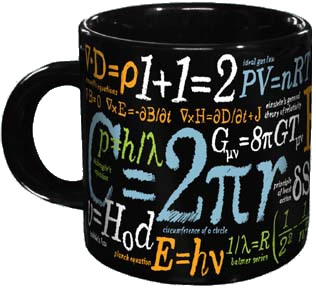
\includegraphics[width=0.15\textwidth]{images/math-mug.jpg}
  \end{center}
\end{frame}

\section{Motivation}

\begin{frame}{A paradoxical situation}  
  \begin{block}{Observation}
    We have powerful tools to mechanize the metatheory of (proof) languages
  \end{block}
  \pause
  \begin{block}{\ldots\ And yet,}
    Workflow of formal mathematics is still largely inspired by legacy
    software development:
    \begin{itemize}
    \item File-based scripts (\textsf{emacs})
    \item Separate compilation (\textsf{make})
    \item Text-based versioning (\textsf{svn}, \textsf{diff}s\ldots)
    \end{itemize}
  \end{block}
  \vspace{0.6em}
  \pause
  \begin{center}
    {\large \it Isn't it time to make these tools metatheory-aware?}
  \end{center}
\end{frame}

\begin{frame}{Motivations}
  \begin{block}{Rigidity of linear edition}
    \begin{itemize}
    \item ((edit; compile)*; commit)* loop does not scale to proofs
    \item Concept freeze inhibits the discovery process
    \item No room for alternate definitions
    \end{itemize}
  \end{block}
  \pause
  \begin{block}{Laxity of textual representation}
    \begin{itemize}
    \item Textual scripts \textsf{diff}s do not reflect the semantics
    \item Not even the syntax
    \end{itemize}
  \end{block}
  \vspace{2em}
  \pause
  {\tiny \ldots\ Maybe it wasn't adapted to software development}
\end{frame}

\begin{frame}{The impact of changes}
  \vspace{0.5em}
  \begin{center}
    \only<1>{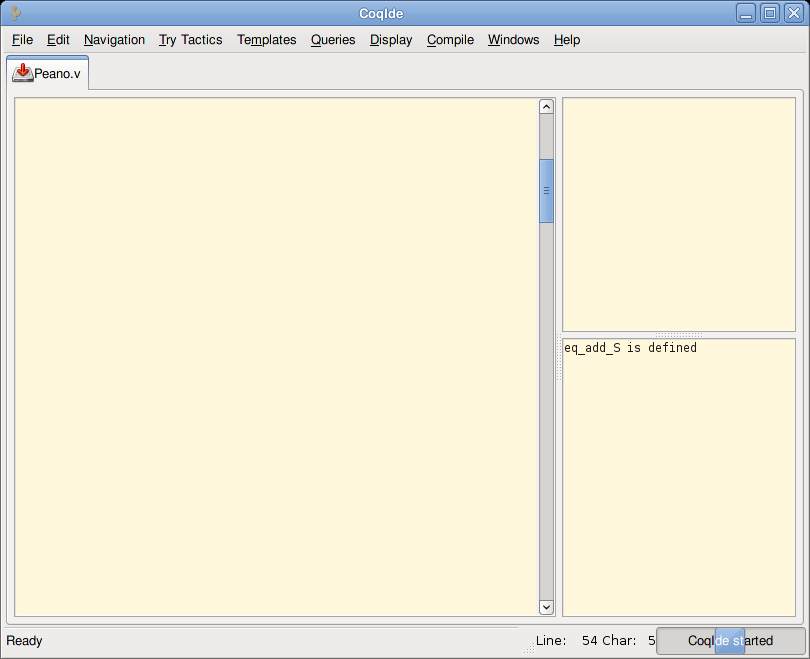
\includegraphics[width=0.75\textwidth]{images/coqide00.png}}%
    \only<2>{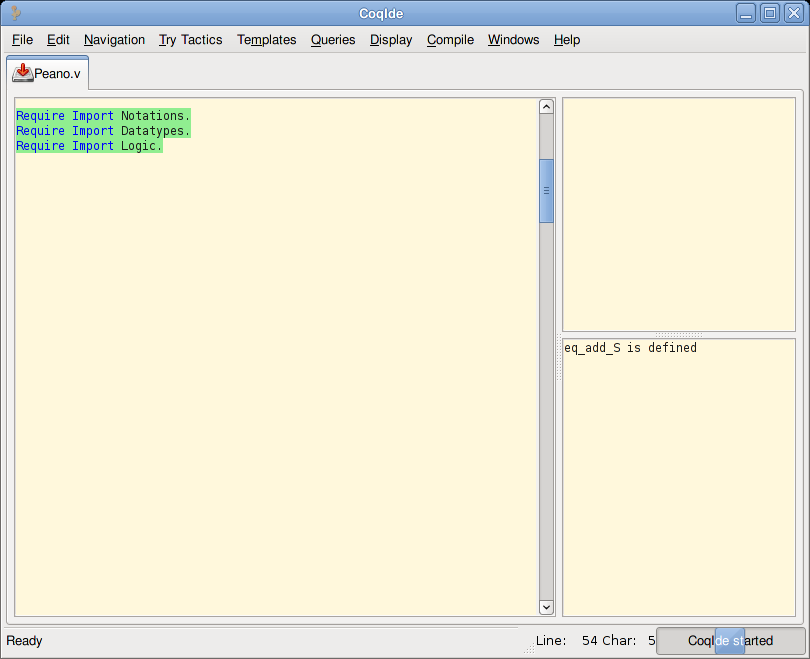
\includegraphics[width=0.75\textwidth]{images/coqide0.png}}%
    \only<3>{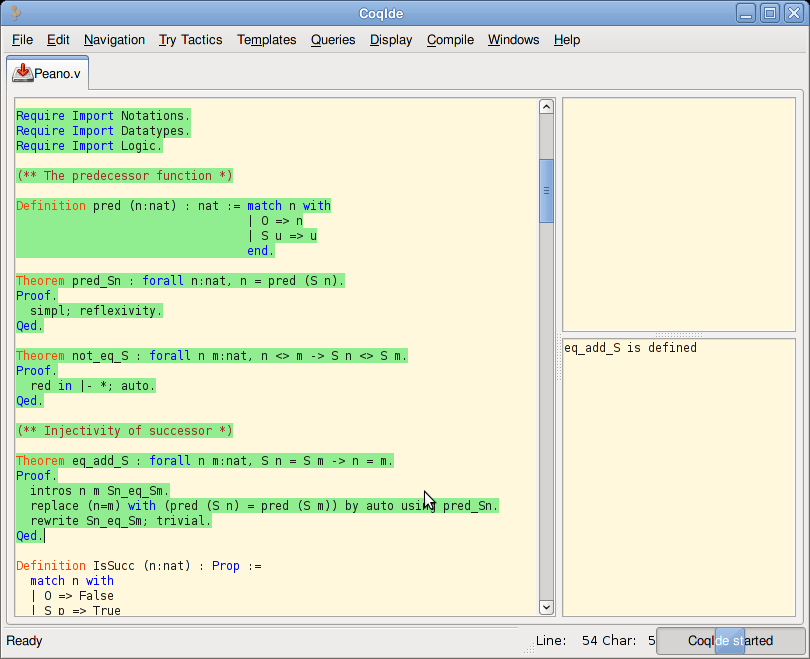
\includegraphics[width=0.75\textwidth]{images/coqide.png}}%
    \only<4>{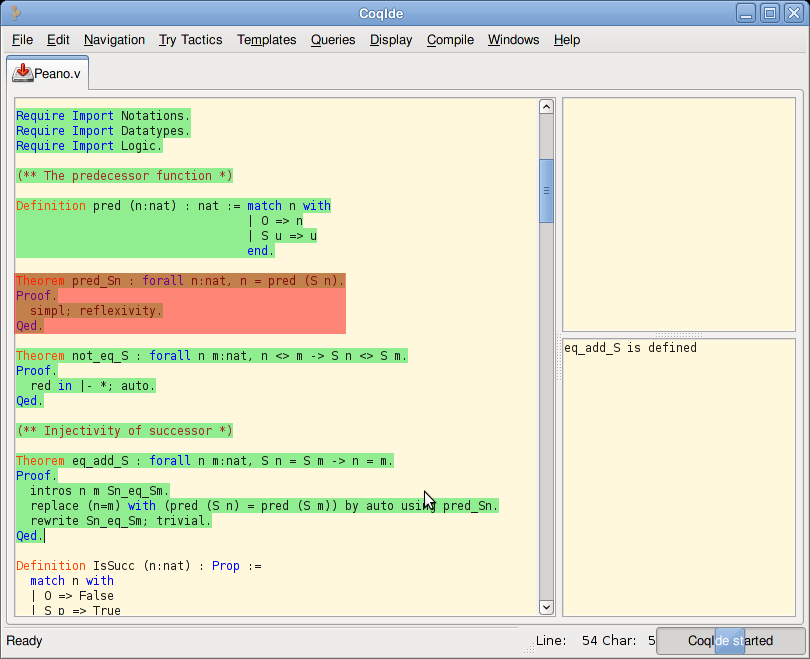
\includegraphics[width=0.75\textwidth]{images/coqide2.png}}%
    \only<5>{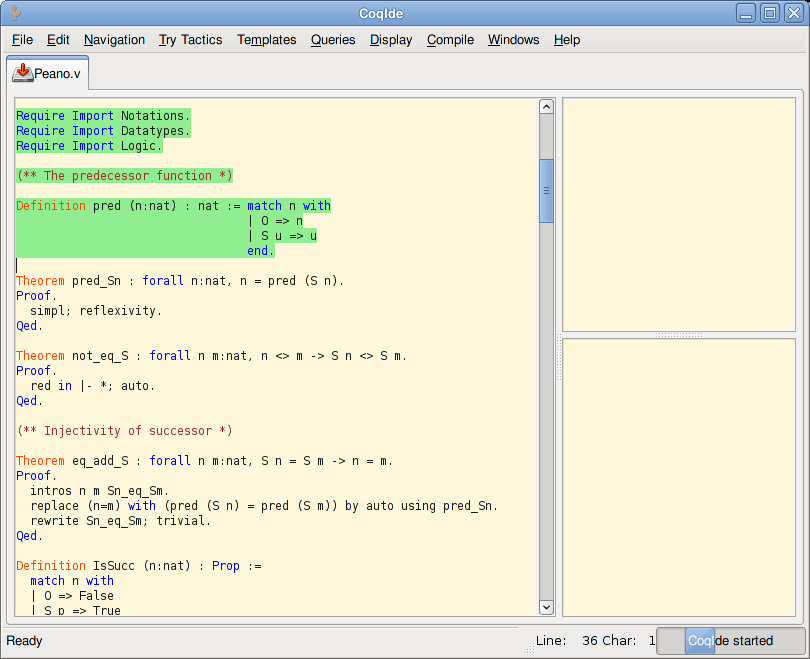
\includegraphics[width=0.75\textwidth]{images/coqide4.png}}%
    \only<6>{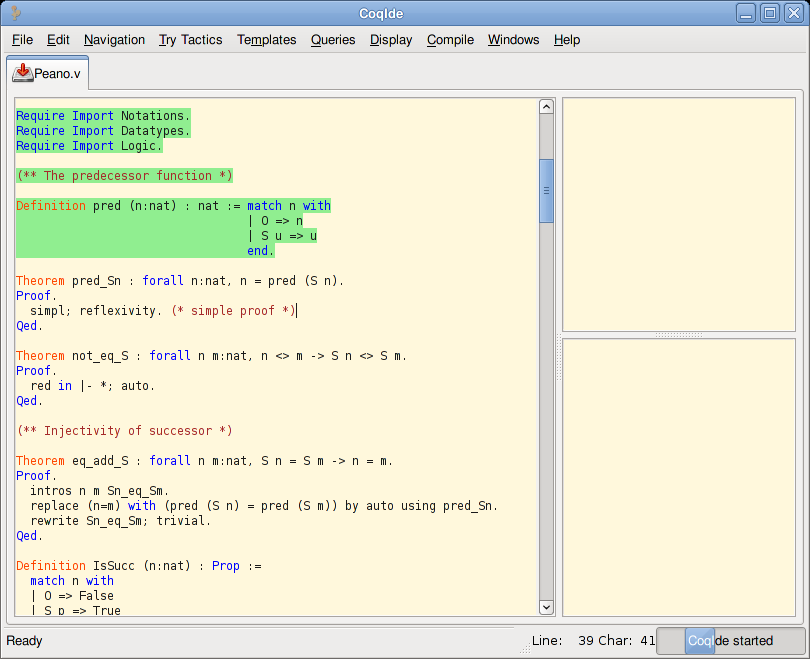
\includegraphics[width=0.75\textwidth]{images/coqide5.png}}%
    \only<7>{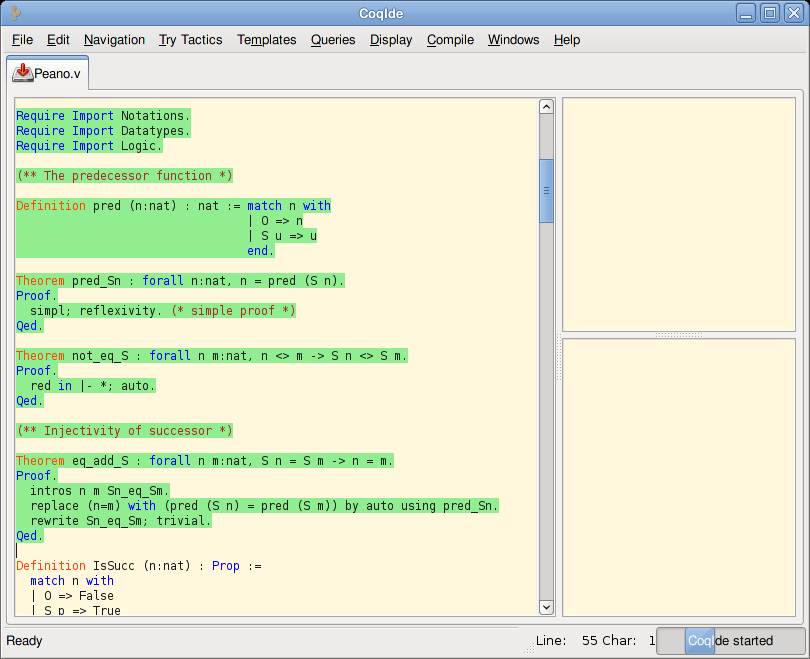
\includegraphics[width=0.75\textwidth]{images/coqide6.png}}%
    \only<8>{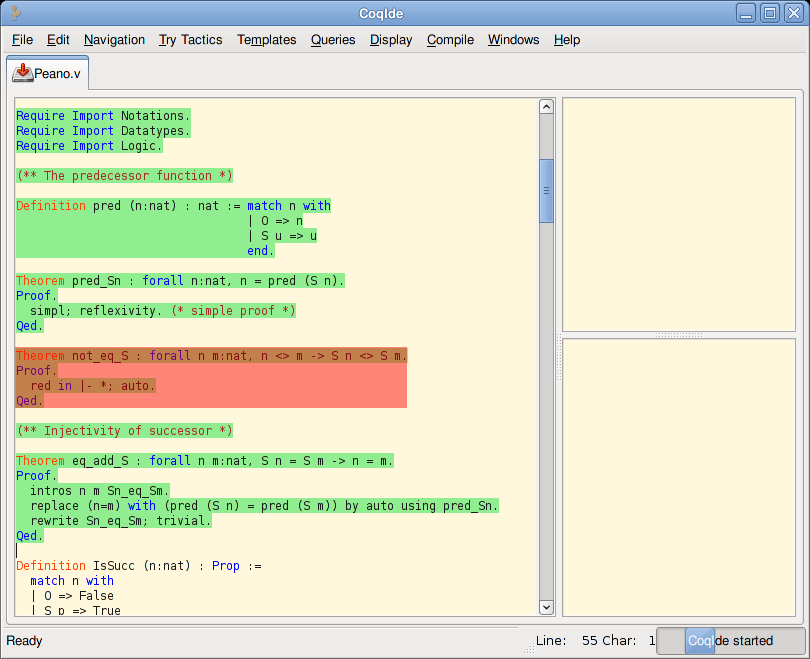
\includegraphics[width=0.75\textwidth]{images/coqide7.png}}%
  \end{center}
  \pause
  \uncover<2->{
    \begin{itemize}
    \item File-based separate compilation
      \pause
    \item Interaction loop with global undo
    \end{itemize}
  }
\end{frame}

\begin{frame}{Methodology}
  \begin{center}
    \only<1-2>{\fbox{\parbox{20em}{\only<2>\alert{version
            management}\\[1em]%
          \fbox{\parbox{18em}{script files\\[1em]%
              \fbox{\parbox{17em}{parsing\\[1em]%
                  \fbox{\parbox{14em}{proof-checking\\} }}}}}}}}%
    \only<3>{\fbox{\parbox{20em}{script files\\[1em]%
          \fbox{\parbox{18em}{\alert{version management}\\[1em]%
              \fbox{\parbox{17em}{parsing\\[1em]%
                  \fbox{\parbox{14em}{proof-checking\\} }}}}}}}}%
    \only<4->{\fbox{\parbox{20em}{\alt<-5>{script files}{user
            interaction}\\[1em]%
          \fbox{\parbox{18em}{parsing\\[1em]%
              \fbox{\parbox{17em}{\alert{version management
                    \only<7->{+ proof-checking}}\\[1em]%
                  \uncover<4-6>{\fbox{\parbox{14.5em}{proof-checking\\}}}}}}}}}}%
  \end{center}
  \begin{itemize}
  \item<4-> AST representation
  \item<5-> Explicit dependency DAG
  \item<7-> Typing annotations
  \item<8-> Incremental type-checking
  \end{itemize}
\end{frame}

\begin{frame}{A core meta-language for incremental type-checking}
  \begin{columns}[t]
    \begin{column}{0.5\textwidth}
      \begin{block}{Expresses}
        \begin{itemize}
        \item (abstract) Syntax
        \item (object-) Logics
        \item Proofs (-terms)
        \end{itemize}
      \end{block}
    \end{column}
    \begin{column}{0.5\textwidth}
      \begin{block}{Features}
        \begin{itemize}
        \item Typing
        \item Incrementality
        \item Dependency
        \end{itemize}
      \end{block}
    \end{column}
  \end{columns}
  \vspace{2em}
  \begin{center}
    \emph{A kernel for a typed version control system?}
  \end{center}
\end{frame}

\begin{frame}{A repository of directories}
  \begin{center}
    \begin{overlayarea}{\textwidth}{14em}
      \begin{center}
        \only<2>{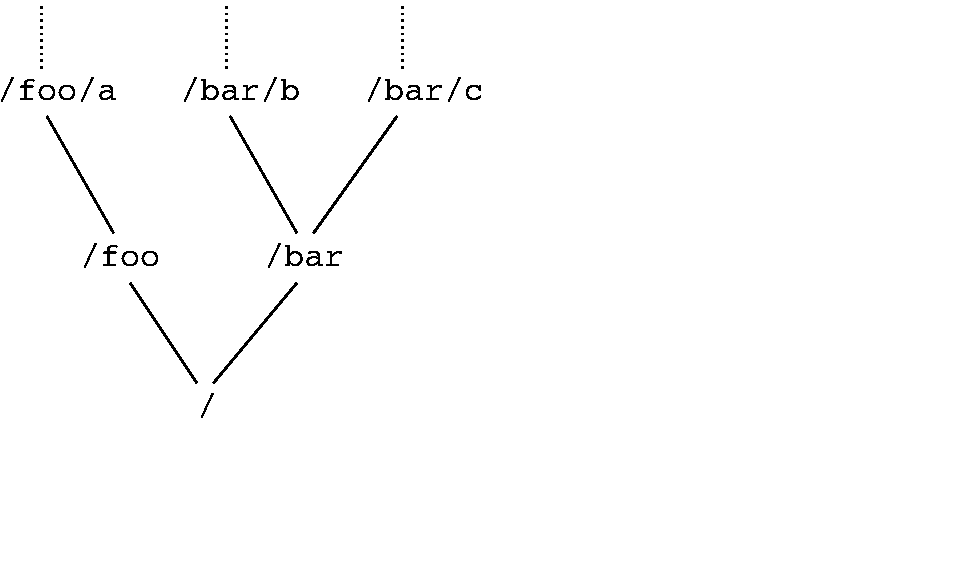
\includegraphics[width=0.85\textwidth]{images/git1.pdf}}%
        \only<3>{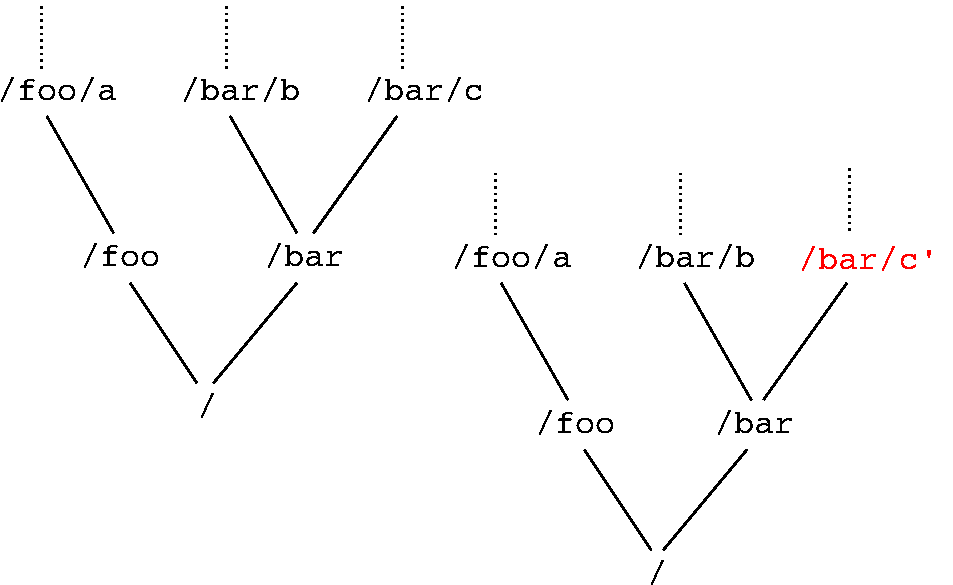
\includegraphics[width=0.85\textwidth]{images/git2.pdf}}%
        \only<4>{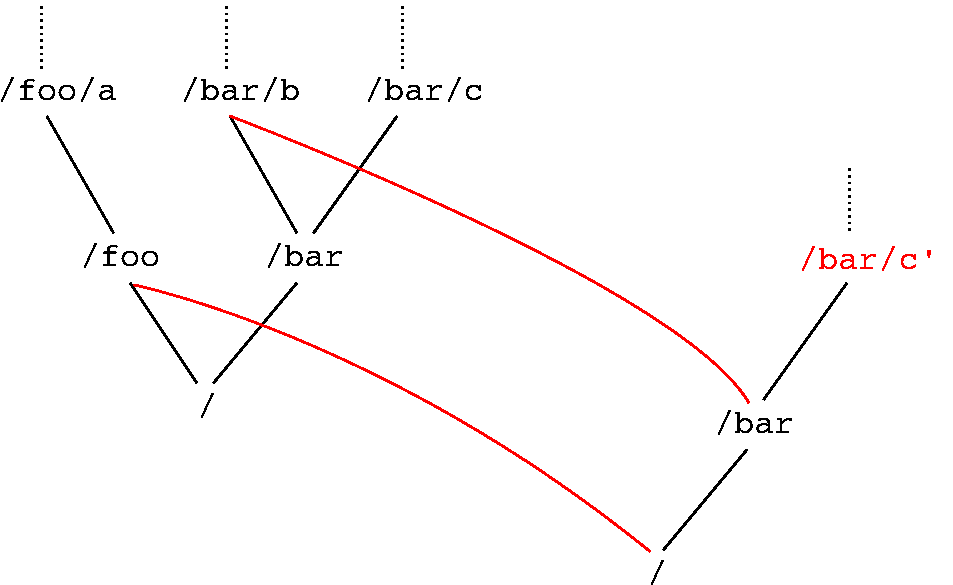
\includegraphics[width=0.85\textwidth]{images/git3.pdf}}%
        \only<5>{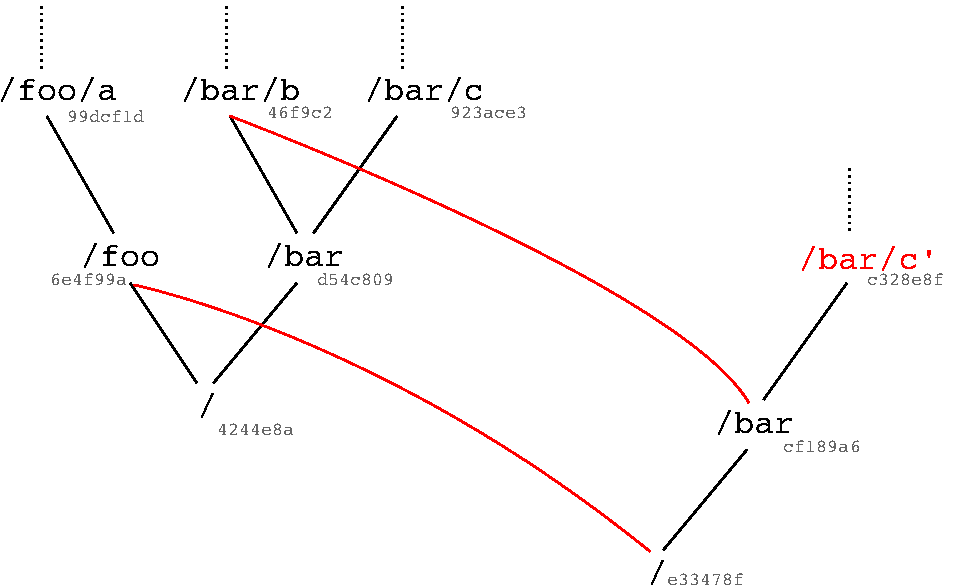
\includegraphics[width=0.85\textwidth]{images/git4.pdf}}%
        \only<6-9>{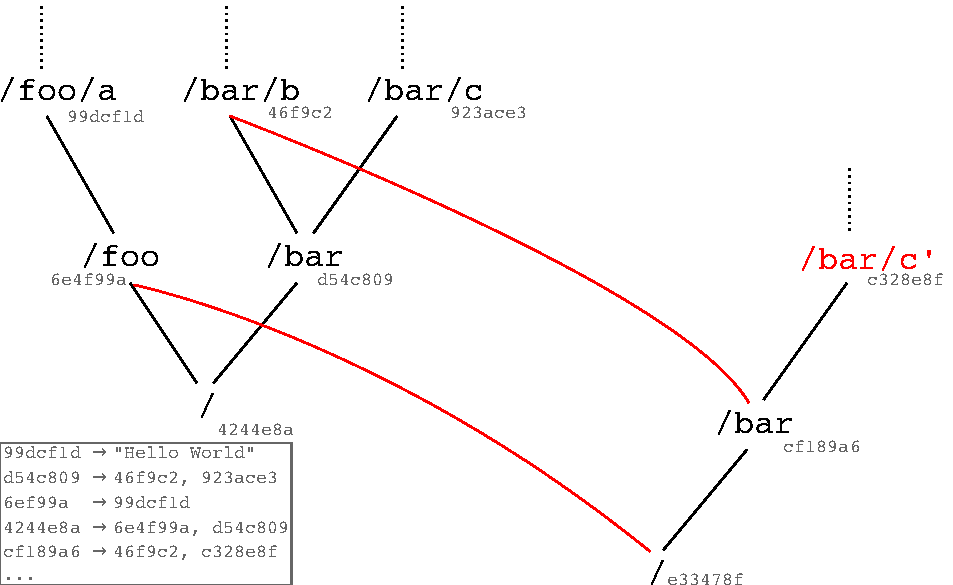
\includegraphics[width=0.85\textwidth]{images/git5.pdf}}%
        \only<10>{
          \begin{center}
            \vspace{5em} {\Large Let's do the same with \emph{proofs}}
          \end{center}
        }%
      \end{center}
    \end{overlayarea}
  \end{center}%
  \begin{itemize}\small %
  \item<7-> ``Content-adressable''%
  \item<8-> Name reflects content%
  \item<9-> Maximal sharing (or hash-consing)%
  \end{itemize}%
\end{frame}

\begin{frame}{A typed repository of proofs}
  \only<1>{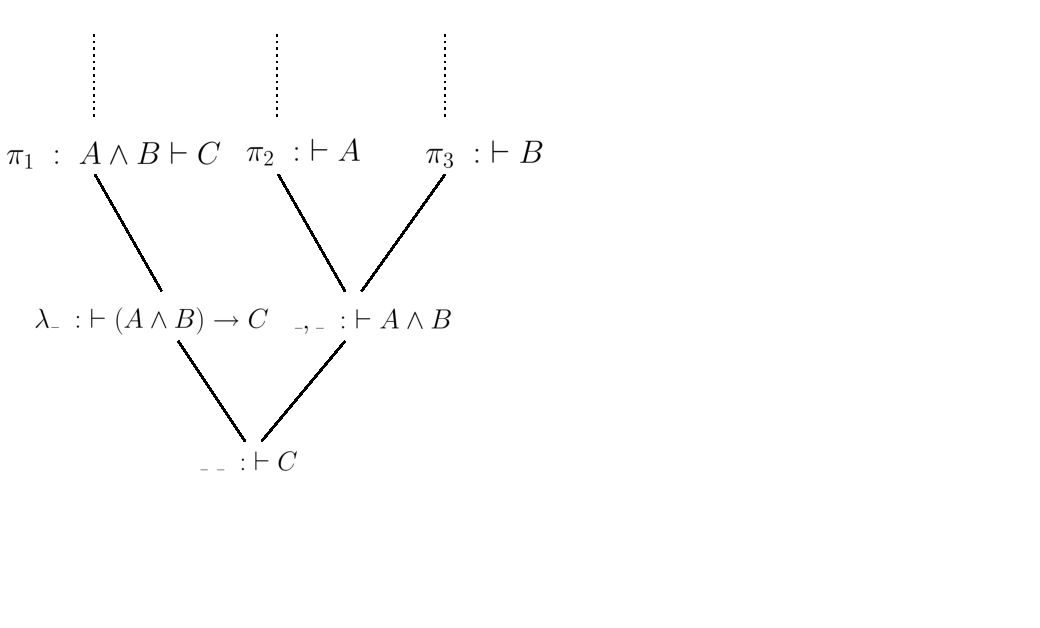
\includegraphics[width=\textwidth]{images/gasp1.pdf}}%
  \only<2>{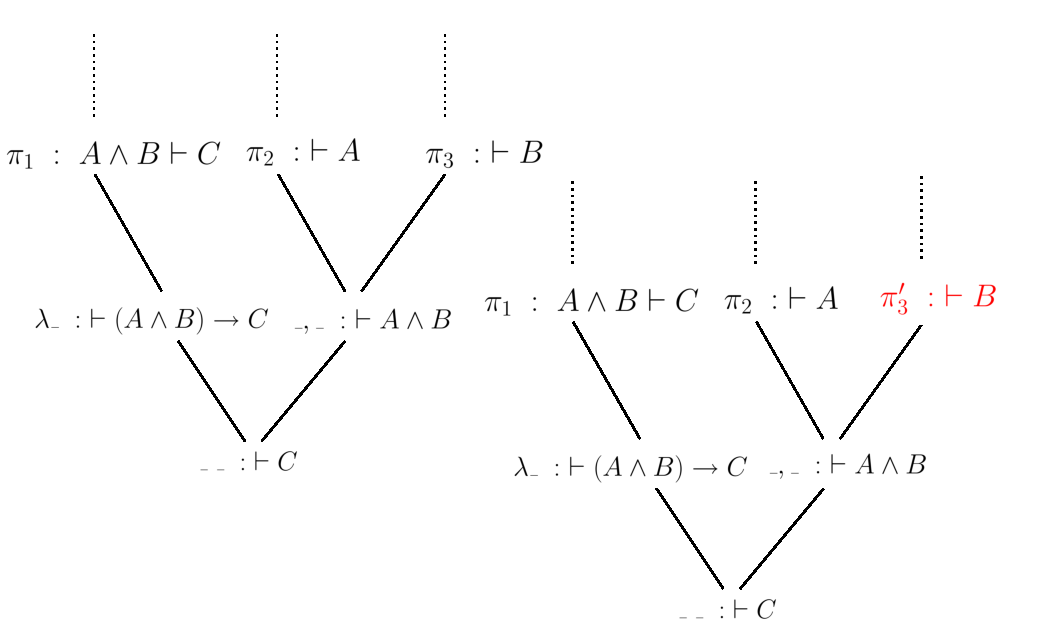
\includegraphics[width=\textwidth]{images/gasp2.pdf}}%
  \only<3>{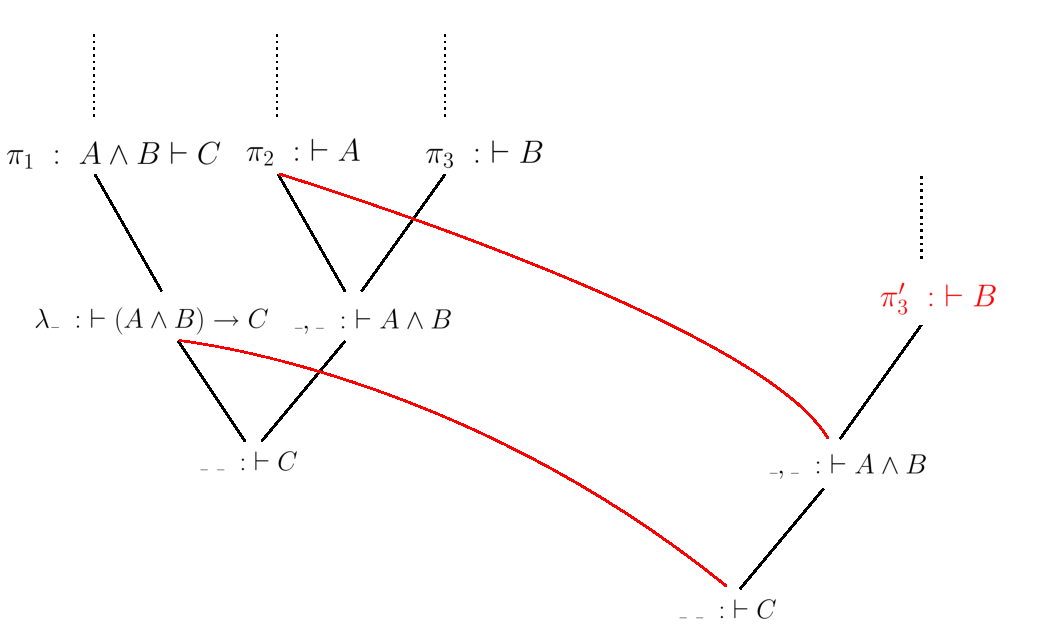
\includegraphics[width=\textwidth]{images/gasp3.pdf}}%
  \only<4>{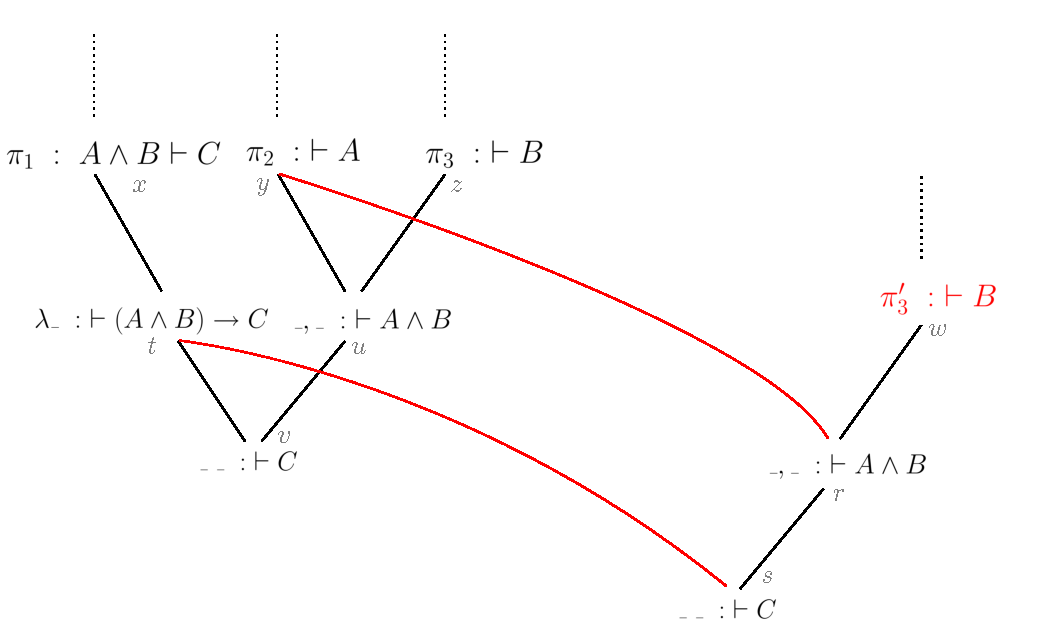
\includegraphics[width=\textwidth]{images/gasp4.pdf}}%
  \only<5>{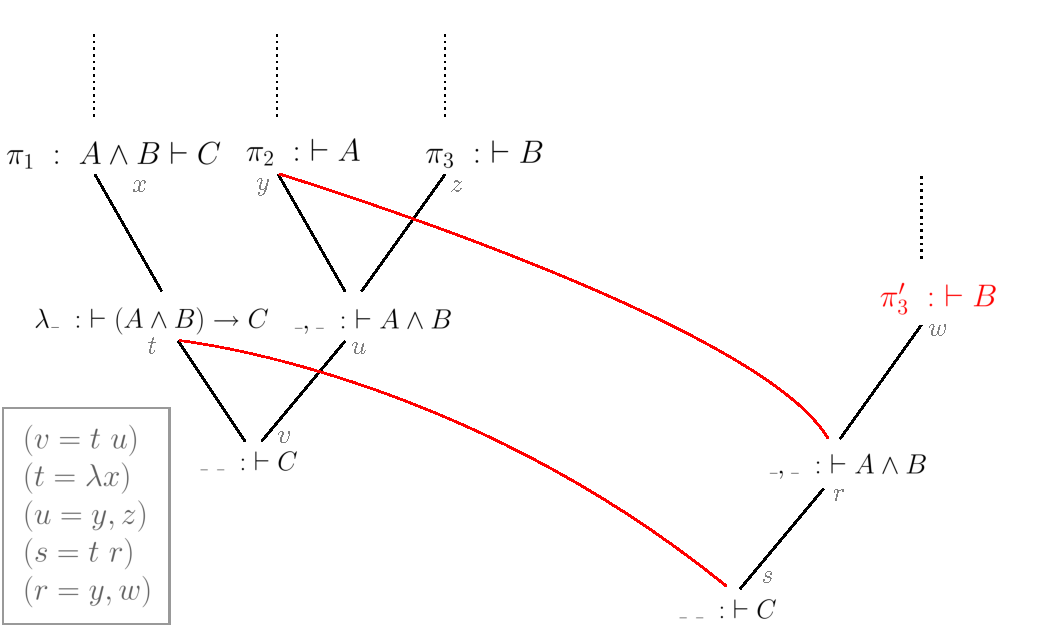
\includegraphics[width=\textwidth]{images/gasp5.pdf}}%
\end{frame}

\begin{frame}{Incremental type-checking, incrementally}%
  \begin{block}{Syntax}%
    \begin{overlayarea}{\textwidth}{3.5em}
      \only<1>{\[ t\ ::=\ [x:t]\cdot t\ |\ (x:t)\cdot t\ |\ x\ |\ t\
        t\ %
        |\ *\] \[\]}%
      \only<2>{\[ t\ ::=\ [x:t]\cdot t\ |\ (x:t)\cdot t\ |\ \alert x\
        |\ %
        \alert{t\ t}\ |\ *\] \[\]}%
      \only<3>{\[ t\ ::=\ [x:t]\cdot t\ |\ (x:t)\cdot t\ |\ \alert a\
        |\ %
        *\]%
        \[ a\ ::=\ x\ |\ a\ x \]}%
      \only<4>{\[ t\ ::=\ [x:t]\cdot t\ |\ (x:t)\cdot t\ |\ a\ |\ *\
        |\ %
        \alert{(x = a)\cdot t}\]%
        \[ a\ ::=\ x\ |\ a\ x \]}%
      \only<5>{\[ t\ ::=\ \alert{[x:t]\cdot t}\ |\ (x:t)\cdot t\ |\
        a\ %
        |\ *\ |\ (x = a)\cdot t\]%
        \[ a\ ::=\ x\ |\ a\ x \]}%
      \only<6->{\[ t\ ::=\ (x:t)\cdot t\ |\ a\ |\ *\ |\ (x = a)\cdot
        t\]%
        \[ a\ ::=\ x\ |\ a\ x \]}%
    \end{overlayarea}
  \end{block}
  \begin{block}{Environments}
      \[ \Gamma\ ::=\ \cdot\ |\ \Gamma [x:t]\only<4>{\ |\
        \alert{\Gamma[x=a:t]}}
      \only<5->{\ |\ \Gamma[x=a:t]} \] 
    \end{block}
    \begin{block}{Judgement}
      \vspace{1em}
        \begin{tabular}{ll} \Large
          $\Gamma\vdash t : u \uncover<7>{\alert{\Rightarrow\Delta}}$
          &
          \only<-6>{`` In environment $\Gamma$, term $t$ has type $u$
            ''}
          \uncover<7>{`` From
            \alert{repository} $\Gamma$, term $t$ of type $u$ \\ &
            \alert{\hspace{1.2em}leads to the new repository $\Delta$}''
          }
        \end{tabular}
    \end{block}
\end{frame}

\begin{frame}{Typing rules}
  \begin{block}{Product}
    \[ \large
    \infer                      % prod
    {\Gamma\vdash t : *\uncover<2->{ \textcolor{gray}{\ \Rightarrow \_}} \and \Gamma[x:t]\vdash u :
      *\uncover<2->{\textcolor{gray}{\ \Rightarrow\Delta}}}
    {\Gamma\vdash(x:t)\cdot u : * \uncover<2->{\textcolor{gray}{\ \Rightarrow\Delta}}}
    \]
  \end{block}
  \pause\pause
  \begin{block}{Init}
    \[\infer{ }
      {\Gamma\vdash x : t \uncover<4->{\textcolor{gray}{\ \Rightarrow\Gamma}}}
      \quad {\small [x:t]\in\Gamma}
      \]
  \end{block}
\end{frame}

\begin{frame}{Typing rules}
  \begin{block}{Equality binder}
    \begin{mathpar}
      \large
      \infer
      {\Gamma\vdash a : u \textcolor{gray}{\ \Rightarrow \_} \and \Gamma[x=a:u]\vdash t :
        *\textcolor{gray}{\ \Rightarrow\Delta} }
      {\Gamma\vdash (x=a)\cdot t : * \textcolor{gray}{\ \Rightarrow\Delta}}
      \quad {\small [y=a:u] \notin\Gamma}
      \and \pause
      \infer
      {\Gamma\vdash t \{y/x\} : * \textcolor{gray}{\ \Rightarrow\Delta}}
      {\Gamma\vdash(x=a)\cdot t : * \textcolor{gray}{\ \Rightarrow\Delta}}
      \quad {\small [y=a:u] \in\Gamma}
    \end{mathpar}
  \end{block}
  \pause
  \begin{block}{Application}
    \[ \infer
      {\Gamma\vdash a : (y:u)\cdot t \textcolor{gray}{\ \Rightarrow\Delta}}
      {\Gamma\vdash a\ x : t \{x/y\} \textcolor{gray}{\ \Rightarrow\Delta}}
      \quad [x : u] \in \Gamma
      \]
  \end{block}
\end{frame}

\begin{frame}{Content-aware names (implementation)}
  Given ``$a$'', how to decide efficiently ``$[y = a : u] \in
  \Gamma$''?
  \pause
  \[ \begin{array}{lllr}
    | \cdot | &:& \vec\kappa \rightarrow \kappa & \text{Hash function}\\
    \equiv    &:& \kappa \rightarrow \kappa \rightarrow \mathbb{B} & \text{Efficient comparison}\\
    \nu       &:& \textsf{unit} \rightarrow \kappa & \text{Fresh key generator}
  \end{array} \]
  \pause
  \begin{mathpar}
    \infer
    {\Gamma\vdash a : u \textcolor{gray}{\ \Rightarrow \_} 
      \and \Gamma[|a|=a:u]\vdash t\{x/|a|\} :
      *\textcolor{gray}{\ \Rightarrow\Delta} }
    {\Gamma\vdash (x=a)\cdot t : * \textcolor{gray}{\ \Rightarrow\Delta}}
    \quad {\small [y=a:u] \notin\Gamma}
    \and
    \pause
    \infer
    {\Gamma\vdash t : *\uncover<2->{ \Rightarrow \_} \and \Gamma[k:t]\vdash u\{x/k\} :
      *\uncover<2->{\textcolor{gray}{\ \Rightarrow\Delta}}}
    {\Gamma\vdash(x:t)\cdot u : * \textcolor{gray}{\textcolor{gray}{\ \Rightarrow\Delta}}}
    \quad{\small k=\nu()}
  \end{mathpar}
  \pause
  \Large
  \[ \Gamma\ :\ \kappa \to \vec\kappa * \tau \]
\end{frame}

\begin{frame}{Further Work}
  \Large
What if we reintroduce {\Huge $[x:t]\cdot t$} ?
\begin{enumerate} \normalsize
\pause
\item Constructive metatheory
\pause
\item A language to express patches?
\end{enumerate}
\end{frame}

\end{document}
